\documentclass[twocolumn,10pt]{article}
\usepackage[a4paper, top=1.0in, bottom=1.0in, left=0.85in, right=0.85in]{geometry}

\usepackage{graphicx}
\usepackage{algorithm}  
\usepackage{algorithmicx}  
\usepackage{algpseudocode}  
\usepackage{amsmath}
\usepackage{url}

\renewcommand{\algorithmicrequire}{\textbf{Input:}}  
\renewcommand{\algorithmicensure}{\textbf{Output:}}  
\graphicspath{{figure/}}

\begin{document}

\date{July 11th, 2017}

\title{\bf Grouper: A Framework for Developing Mobile Application Using Secret Sharing and Untrusted Servers}

\author{
	Meng Li, 201620728  
	\\ Supervisor: Yasushi Shinjo
}

\maketitle

\section{Introduction}
Conventional client-server mode applications requires central servers for storing shared data. The users of such mobile applications must fully trust the central server and their application providers. If a central server is compromised by hackers, user information may be revealed because data is often stored on the server in cleartext. Users may lose their data when service providers shut down their services. 

To solve this problem, Mylar\cite{popa2014building}, a Web application framework use browser extension to encrypt and decrypt user data only in client. In this paper, we are are implementing a mobile application framework, Grouper, that is not relied on trusted central servers.

A popular approach to address the central server problem is using P2P(Peer to Peer) to transfer user data between devices. However, there is an obvious problem in such a P2P approach. Data transfer can only be finished during two devices are online at the same time. Another problem is that the number of P2P connections becomes large  fast as the number of users increases. 

Unlike P2P systems, we use multiple untrusted servers for data transfer. Data is divided into several pieces by secret sharing scheme and uploaded to diverse servers. Each server can only keep a piece of data temporarily, we call it share. A share will be deleted after a period of time. These ensure that user data cannot be cracked easily. In addition, all devices of group members keep a complete data set, and data can be recovered even untrusted servers shut down.

\section{Design}

We design this framework on iOS platform at first. We are aiming at developing applications which is not relying on trusted central server using our Grouper framework. 

\subsection{Overview}
Applications by Grouper can synchronize data between members of a group. In our situation, each group member holds a device. Thus, Grouper should provides main functions.

\begin{itemize}
	\setlength{\itemsep}{1pt}
	\setlength{\parskip}{0pt}
	\setlength{\parsep}{0pt}
	\item Data synchronization: the group member create an object and others synchronize this object.
	\item Group management: the group owner create a group in his device and invites other members to his group.
\end{itemize}

\subsection{Data Synchronization}

In Grouper, a device use Secret Sharing scheme to divide a message into several shares and upload them to multiple untrusted servers. Other devices download shares and recover shares to original message by Secret Sharing scheme.

\subsubsection{Shamir's Secret Sharing}
Secret sharing plays an indispensable role in protecting user data from getting lost or destroyed. In a secret sharing scheme, a dealer securely shares a secret with a group of members by generating $n$ shares using a cryptographic function\cite{smith2013layered}. At least $k$ or more shares can reconstruct the secret, but $k-1$ or fewer shares can obtain nothing about the secret\cite{pang2005new}. We describe this scheme as a function $f(k, n)$, where $n$ is the number of all shares, and $k$ is the threshold to combine shares.  We use Shamir's secret sharing that  is a popular technique to implement threshold schemes.

\subsubsection{Multiple Untrusted Servers}

We design Grouper based on data synchronization through multiple untrusted servers rather than a single server. There are three principles in our proposal. 

Firstly, a server transfers data as similar to a router, but does not keep it permanently. Most current popular client-server applications store their user data on several central servers, and the user's data will not be deleted unless the user deletes his account. Grouper uses untrusted servers as a bridge for transferring data. Consider that a group includes three members: Alice, Bob and Carol. Alice creates a new record in her device, this record is uploaded to untrusted servers, and the record on servers will be deleted after Bob and Carol download it from servers.

Secondly, a server keeps data temporarily. We define a period of time in which data can be kept in a server, we call it interval time. In this paper, we set this period to 1 hour for our example situations. The record Alice uploaded to untrusted servers can exist for 1 hour. After 1 hour since uploaded, this record will be deleted. Alice requires to upload this record again to serves until all of other members have downloaded successfully. The longer keeping period means the higher risk of data reveal. We will find suitable periods as the number of group members, security requirement and others. 

Thirdly, servers do not know the cleartext of data. Keeping data temporarily cannot ensure data security, because servers know the cleartext of data in this temporary period. For this problem, developers often encrypt data before uploading to servers, and this needs a decryption key to decrypt data in other devices. In order to distribute the decryption key, users should share it by themselves. In Grouper, we do not encrypt data but we use a secret sharing scheme as described in Section 2.2. Servers do not know the cleartext of a share generated by a secret sharing scheme.

\begin{figure}[t]
	\centering
	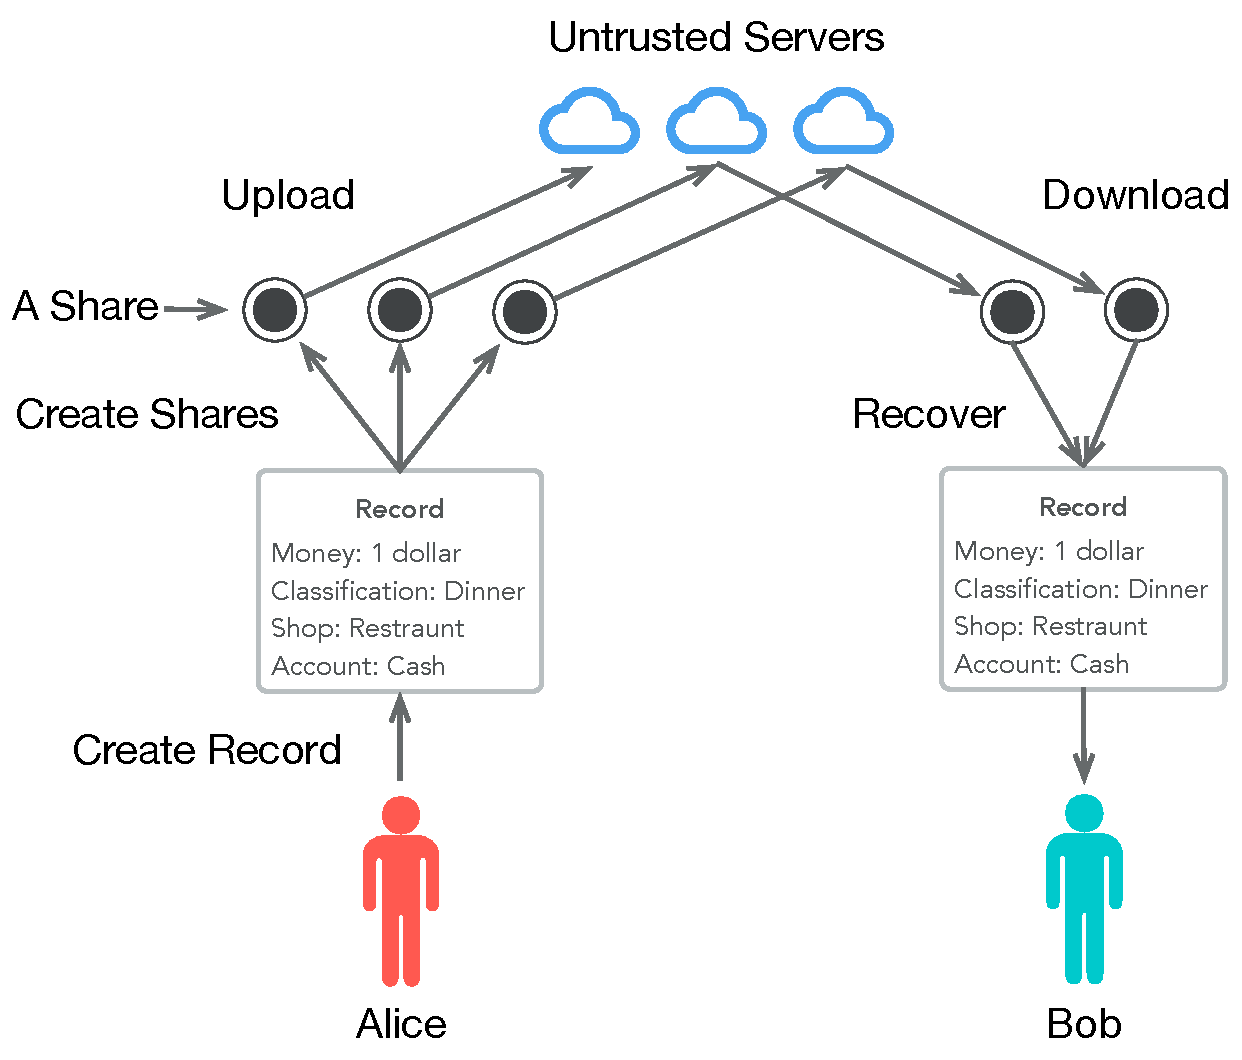
\includegraphics[scale=0.38]{sync_flow}
	\caption{Flow of synchronization.}
\end{figure}

Figure 1 describes our synchronization flow based on these three principles. At first, Alice adds a record and Grouper creates three shares by a secret sharing scheme where $n$ is three and $k$ is two. Next, Grouper uploads those shares to three untrusted servers. When Bob is online, Grouper in Bob's device downloads two shares from servers and recovers the new record created by Alice. In this situation, Grouper can recover the record after getting two or more shares. In this process, each server is separated from other servers, and cannot access to other servers. This means these servers cannot recover user data because they do not have permission to access other untrusted servers. In our proposal, only group members have permission to access these untrusted servers.

\subsection{Group Management}

\subsubsection{Creating Group}

A group is created by its owner. For example, Alice is a group owner. Alice should prepare her own user information including email and name at first. Then, she should add multiple untrusted servers by submitting group ID and group name. Here, the group ID and group name are assigned by Alice and they should be same in all untrusted servers of this group. 

At last, Alice should initialize this group on all untrusted server by submitting her node identifier. The node identifier which can represent Alice's device, is generated by Group randomly when the app is launched at first time.  In each untrusted server, its Web service initializes this new group and returns a master key including the highest privilege to Alice. Alice can add other members to an untrusted server by the master key.

\subsubsection{Inviting Member}

After creating a group, Alice can invite her friends to her group. As a friend of Alice, Bob should also prepare his user information at first. Figure 3 shows the procedure to add a new member to a group. Alice can only invite Bob by a face-to-face way rather than connection via Internet using central server. Before inviting, Grouper establish connection between Alice's and Bob's devices. Firstly, Bob's device sends his user information and node identifier to Alice's device. Alice saves Bobs's user information and node identifier to her device. Secondly, Alice register Bob on multiple untrusted server by submitting Bob's node identifier. Thirdly, untrusted servers returns Bob' access key to Alice. Lastly, Alice send Bob's access key, server related information and all users' information she has to Bob.

\begin{figure}[t]
	\centering
	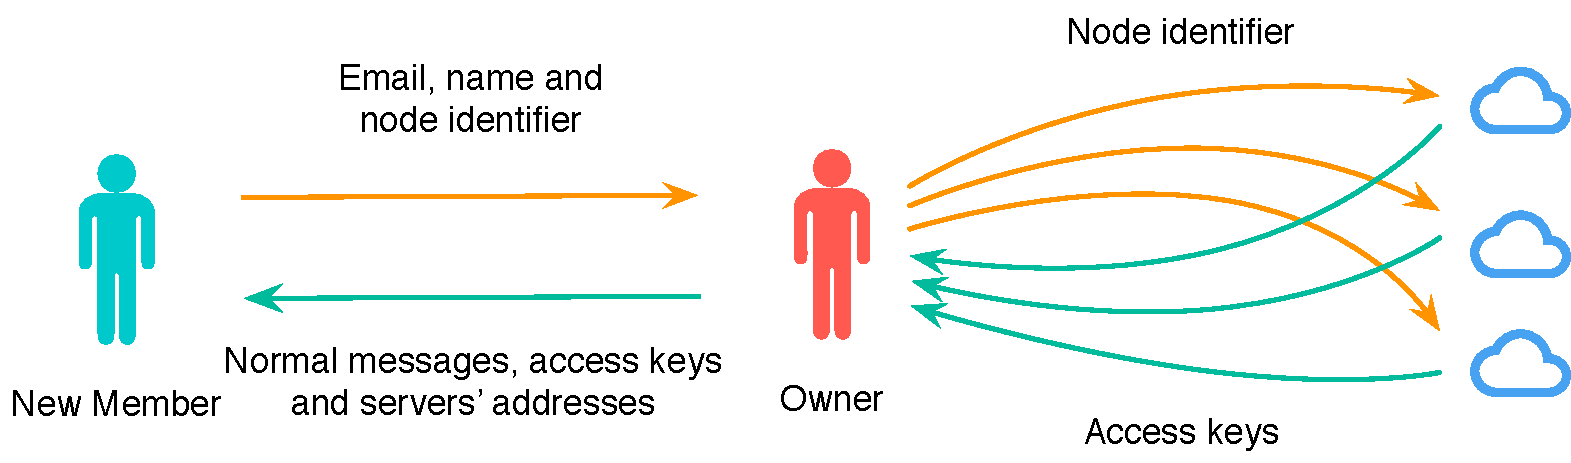
\includegraphics[scale=0.38]{add_member}
	\caption{Adding a new member.}
\end{figure}

\subsection{Reliable Synchronization}
Grouper should provide a reliable synchronization service. For example, Alice is a user in a group and creates a new record in her device. All of other members in a group should synchronize this record, even if this record may be deleted by untrusted servers after a period of time. We call this problem \emph{reliable synchronization}.

Figure 2 describes an unreliable situation that data cannot be synchronized. Alice sends a new record to untrusted servers and Bob downloads it successfully within the interval time. Carol becomes online after the interval time and fails to download shares of this record because they have been deleted by servers. To solve this problem, Alice should upload her new record again until Carol downloads it successfully.

\begin{figure}[t]
	\centering
	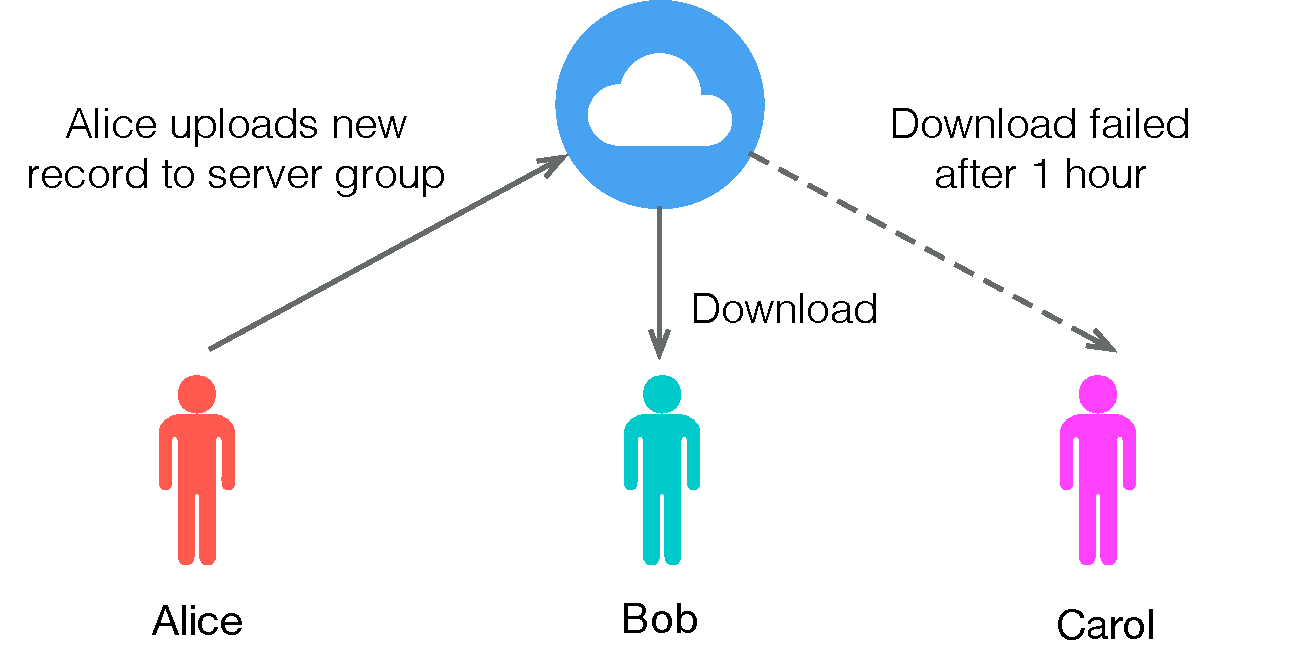
\includegraphics[scale=0.38]{unreliabe_sync}
	\caption{Unreliable synchronization.}
\end{figure}

To solve this problem, we reference the basic reliable multicasting scheme in distribute systems. Messages in this scheme should have sequence number which is added one by one, to indicate the sending order of those messages. For example, the sender of a group send a message No.25 and all of the receivers receive the message No.25 successfully. When the receivers receive new message No.25, they will compare No.25 with the newest sequence number in their persistent store. One of the receivers finds that his newest sequence number is No.23, that means he missed the message No.24. Thus, when they send feedback to the receiver, he will report that he missed the message No.24. At last, the sender will send the missed message to him.

\section{Implementation}

\subsection{Sync Entity}

Applications by Grouper should use Core Data as it's persistent store solution, because our data synchronization is based on the \emph{Sync} framework which is relying on Core Data. Developers should design the entities for Core Data to store their application related data.

Grouper provides an entity called \emph{Sync Entity} as the parent entity of your application entities. In a sync entity, there are some basic attributes.

\begin{table}[]
	\centering
	\caption{Attributes of Sync Entity}
	\begin{tabular}{lll}
		\hline
		\textbf{Attribute} & \textbf{Type} & \textbf{Explanation}         \\ \hline
		createAt           & Date          & Create date of this entity   \\ \hline
		creator            & String        & Creator of this entity       \\ \hline
		remoteID           & String        & Remote ID for Sync framework \\ \hline
		update             & String        & Updater of this entity       \\ \hline
		updateAt           & String        & Update date of this entity   \\ \hline
	\end{tabular}
\end{table}

These attributes are necessary for data synchronization. Only by inheriting the sync entity can an application entity synchronize between devices of a group.

\subsection{Sync Message}

To transfer data between devices, we reference the protocol of email and design our own \emph{Sync Message}.

In fact, a sync message is a JSON string that contains the sync entity related information and the way to handle it in receiver’s device. There are 4 types of sync message, they are update message, delete message, confirm message and resend message. Both update message and delete message need resend because they contain sync entity related information. We call them normal message. Both confirm message and resend message contain control information about reliable multicast and need not resend. We call them control message.

When a user creates a new entity or modifies some attributes of an existed entity, the application should send an update message that contains the JSON string of this entity to all group members.

When a user deletes an existed entity, the application should send a delete message that contains the object ID of this entity to all group members.

For reliable multicasting, when the application is launched, it should check the send time if the last confirm message. If it sent before the interval time, the application should send a new confirm message that contains the sequences of all messages which are sent by this devices before, to all group members.

When the device of a group member receives a confirm message, it should check the sequences. If some of them are nonexistent in its' persistent store, the application should send a resend message that contains the nonexistent part of the sequences.

\subsection{Architechture}
Grouper consists of a client framework for developing iOS application and a Web service running on multiple untrusted servers. In Section 2, we have introduced how to share strings with other deices via multiple untrusted servers. In this section, we describe persistent store and data synchronization. Grouper stores all data on mobile devices with an object-oriented way.

\subsubsection{Web Service}
Grouper needs its own Web service rather than using commercial general cloud services like Amazon S3, Google Cloud for following reasons:

\begin{itemize}
	\setlength{\itemsep}{1pt}
	\setlength{\parskip}{0pt}
	\setlength{\parsep}{0pt}
	\item The Web service supports reliable synchronization.
	\item The Web service ensures that shares are deleted after a prescriptive time.
	\item The Web service allows only group members who have access keys to download shares.
\end{itemize}

Our Web service runs on the Tomcat server that is an open source implementation of the Java Servlet, JavaServer Pages, Java Expression Language and Java WebSocket technologies. We use the Spring MVC, a  Web model-view-controller framework, to create our RESTful API, and Hibernate, an open source Java ORM framework, to save and operate object in the Web service. 

Our Web service include three entities. They are \emph{Group}, \emph{User} and \emph{Transfer}. The \emph{Group} entity saves the unique identifier, group name and its owner. The \emph{User} entity save the node identifier of a user, access key for this user, and group of this user. The \emph{Transfer} entity saves a share generated with a secret sharing scheme, the time when the user uploads it and its creator. For each user, there is a unique access key for him in an untrusted server. Thus, only this user can modify or remove what he uploaded to this server. For a group, one of a user is its owner who has the highest privilege of this group.

In a word, our web service provides RESTful API to transfer data with clients, and it keeps shares from devices temporarily.

\subsubsection{Client}

Grouper provides a client framework by Objective-C language to developing applications on iOS, macOS, watchOS and tvOS. 
 
Figure 4 describes the architecture of client framework. It is based on such frameworks.   

\begin{itemize}
	\setlength{\itemsep}{1pt}
	\setlength{\parskip}{0pt}
	\setlength{\parsep}{0pt}
	\item Grouper used \emph{Multipeer Connectivity}\cite{mc},  a official peer-to-peer communication framework provided by Apple, to transfer data between devices by a face-to-face way.
	\item Grouper uses \emph{Core Data}\cite{coredata}, a official ORM framework provided by Apple, to manage the model layer objects.\emph{Core Data} provides generalized and automated solutions to common tasks associated with object life cycle and object graph management, including persistence.
	\item Grouper uses \emph{Sync}\cite{sync}, a modern JSON synchronization framework for \emph{Core Data}, to create JSON strings and synchronize object from JSON strings.
	\item Grouper uses \emph{c-SSS}\cite{c-sss}, an implementation of Shamir's secret sharing in the C language, to create shares and recover shares.
	\item Grouper uses \emph{AFNetworking}\cite{afnetworking}, a delightful networking library by Objective-C language, to revoke the RESTful API provided by our Web services. 
\end{itemize}

 \begin{figure}[t]
	\centering
	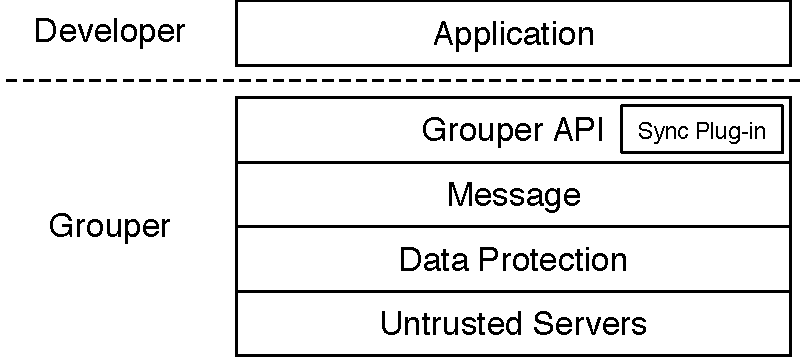
\includegraphics[scale=0.35]{architecture}
	\caption{Architecture of the iOS application.}
\end{figure}

\section{Related Work}

DepSky\cite{bessani2013depsky} is a system that stores encrypted data on servers and runs application logic. DepSky provides a storage service that improves the availability and confidentiality by using commercial storage services. \emph{Cloud-of-Clouds} is the core concept in DepSky. It represents that DepSky is a virtual storage, and its users invoke operations in several individual severs. DepSky keeps encrypted data in commercial storage services and do application logic in individual servers. In Grouper,  untrusted servers undertake responsibility of temporarily data storage and message delivery with server-side computation.

Mylar\cite{popa2014building} stores encrypted and sensitive data on a server, and decrypts this data only in users’ browsers. Developers of Mylar use its API to encrypt a regular(non-encrypted) Web application, and users decrypt data by a browser extension. Like in Grouper, applications in Mylar can control how user data is shared. Mylar builds its system on a browser with extension while Grouper uses mobile devices.

There are many applications and frameworks that use untrusted networks and servers. Compared to them, Grouper uses secret sharing and temporary data storage with untrusted servers to protect user data. Using secret sharing is more convenient and faster than using data encryption because clients need not to distribute decryption keys and perform heavy encryption computation.

\section{Conclusion}

This paper introduces Grouper, a group finance manager that synchronizes data among mobile devices with multiple untrusted servers. Grouper uses secret sharing and temporary data storage services. Grouper consists of clients that run an iOS application and multiple untrusted servers that run a Web service. Each server of Grouper does not know the others and keeps one piece of the shares generated by secret sharing temporarily to protect user data. We connect clients and multiple untrusted servers by a REST API. We are developing a robust protocol of reliable synchronization using multiple untrusted servers.

\bibliographystyle{unsrt}
{
	\footnotesize
	\bibliography{ref}
}

\end{document}
